\documentclass[tikz,border=4pt]{standalone}
\usepackage{amsmath}
\begin{document}
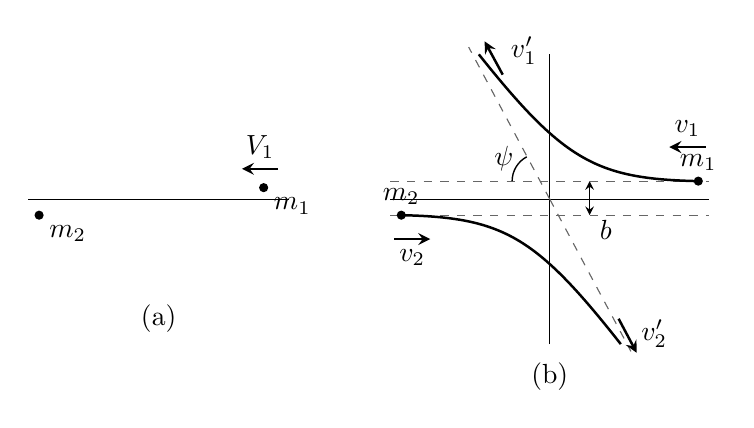
\begin{tikzpicture}[>=stealth, thick, scale=0.92]
  % Left: Lab frame
  \begin{scope}[xshift=-4.3cm]
    \draw[line width=0.4pt] (-1.5, 0) -- (2.1, 0);
    % m2 at rest
    \fill (-1.35, -0.22) circle (1.8pt) node[below right] {$m_2$};
    % m1 approaching from right
    \fill (1.75, 0.16) circle (1.8pt) node[below right] {$m_1$};
    \draw[->, line width=0.9pt] (1.95, 0.42) -- (1.45, 0.42);
    \node[above] at (1.7, 0.42) {$V_1$};
    \node at (0.3, -1.65) {(a)};
  \end{scope}

  % Right: CM frame
  \begin{scope}[xshift=1.4cm]
    % Axes / reference lines
    \draw[line width=0.4pt] (-2.2, 0) -- (2.2, 0);
    \draw[line width=0.4pt] (0, -2.0) -- (0, 2.0);
    \draw[dashed, line width=0.4pt, black!60] (-2.2, 0.25) -- (2.2, 0.25);
    \draw[dashed, line width=0.4pt, black!60] (-2.2, -0.22) -- (2.2, -0.22);

    % Asymptotes of scattered directions (angle psi ~ 62 deg from -x)
    \draw[dashed, line width=0.4pt, black!60] (0, 0) -- (-1.12, 2.1);
    \draw[dashed, line width=0.4pt, black!60] (0, 0) -- (1.12, -2.1);

    % Trajectory 1 (m1 coming from right, deflected up-left)
    \draw[line width=0.9pt] (2.05, 0.25) .. controls (0.65, 0.28) and (0.2, 0.52) .. (-0.98, 2.0);
    \fill (2.05, 0.25) circle (1.8pt) node[above] {$m_1$};
    \draw[->, line width=0.9pt] (2.15, 0.72) -- (1.65, 0.72);
    \node[above] at (1.9, 0.72) {$v_1$};
    \draw[->, line width=0.9pt] (-0.65, 1.72) -- (-0.90, 2.18);
    \node[right] at (-0.68, 2.05) {$v'_1$};

    % Trajectory 2 (m2 coming from left, deflected down-right)
    \draw[line width=0.9pt] (-2.05, -0.22) .. controls (-0.65, -0.25) and (-0.2, -0.5) .. (0.98, -2.0);
    \fill (-2.05, -0.22) circle (1.8pt) node[above] {$m_2$};
    \draw[->, line width=0.9pt] (-2.15, -0.55) -- (-1.65, -0.55);
    \node[below] at (-1.9, -0.55) {$v_2$};
    \draw[->, line width=0.9pt] (0.95, -1.65) -- (1.20, -2.12);
    \node[right] at (1.12, -1.85) {$v'_2$};

    % Impact parameter b
    \draw[<->, line width=0.4pt] (0.55, -0.22) -- (0.55, 0.25);
    \node[right] at (0.55, -0.42) {$b$};

    % Scattering angle psi
    \draw[line width=0.5pt] (-0.52, 0.25) arc (180:118:0.38);
    \node[above left] at (-0.36, 0.25) {$\psi$};

    \node at (0, -2.45) {(b)};
  \end{scope}
\end{tikzpicture}
\end{document}
